\documentclass[a4paper]{article}
\usepackage{lipsum}
\usepackage{url}
\usepackage{graphicx}
\usepackage{listings}
\lstset{language=Python}
\usepackage[margin=3cm]{geometry}
\graphicspath{ {images/} }
\usepackage{afterpage}
\usepackage[]{algorithm2e}
\usepackage{float}
\usepackage{multicol}
\usepackage{CJKutf8}

%Custom Commands
\newcommand{\Pokemon}{Pok\'{e}mon}
\newcommand{\Pokeapi}{Pok\'{e}api}

\begin{document}

\pagenumbering{gobble}

\begin{center}
	
\includegraphics[height=3cm]{UoNLogo.png}

	\vfill
	\Huge{\textbf{Benjamin Joshua Charlton}}
	\vfill
	\LARGE{	ID Number: 4262648 \\
			Supervisor: Professor Robert John \\
			Module Code: G53IDS
			\vfill
			2018/04
			\vfill}
	\afterpage{\null\newpage}
\end{center}


\begin{titlepage}
	\newcommand{\HRule}{\rule{\linewidth}{0.5mm}}
	\center{}

    %Headings
	
\includegraphics[height=3cm]{UoNLogo.png}\\[0.5cm]
	\Large{Computer Science with Artificial Intelligence MSci}\\[0.5cm]
	\large{G53IDS - Individual Dissertation}\\[0.5cm]

    %Title
	\HRule{}\\[0.4cm]
	{\huge\bfseries Applying Evolutionary Algorithms to \Pokemon{} Team Building}\\[0.4cm]
	\HRule{}\\[1.5cm]

	Submitted April 2018, in partial fulfilment of the conditions for the award of the degree Computer Science with Artificial Intelligence MSci
	\vfill

    %Authors
	\begin{minipage}{0.4\textwidth}
		\begin{flushleft}
			\large
			\textit{Author}\\
			Benjamin \textsc{Charlton}\\
            psybc3@nottingham.ac.uk\\
            4262648
		\end{flushleft}
	\end{minipage}
    \begin{minipage}{0.4\textwidth}
		\begin{flushright}
			\large
			\textit{Supervisor}\\
			Prof.\@ Bob \textsc{John}\\
            Robert.John@nottingham.ac.uk
		\end{flushright}
	\end{minipage}


	\vfill
	School of Computer Science \\
	University of Nottingham \\

	\vfill
	I hereby declare that this dissertation is all \\
	my own work, except as indicated in the text:
	\\ [1cm]
	Signature:\rule{6cm}{0.15mm}

    %Date
	\vfill\vfill\vfill
	{\large24\textsuperscript{th} April 2018}
	\vfill

\afterpage{\null\newpage}
\normalsize{}
\end{titlepage}

\setcounter{page}{1}
\pagenumbering{roman}

\section*{Abstract}
\addcontentsline{toc}{section}{Abstract}
\begin{itemize}
    \item Short overview of the entire project
\end{itemize}
The aim of this dissertation is to show AI search methods can be used to help pre-game decision making tasks such as team and deck building.
As AI game playing moves towards more complicated games the idea of how to tackle these pre-game choices will come up whether in choosing the deck list in a collectable card game or item load outs in a turn based strategy game.
\par
The focus of this project is the team building aspect of the \Pokemon{} games and how it can be tackled using an evolutionary algorithm.
\vfill
\section*{Acknowledgements}
\addcontentsline{toc}{section}{Acknowledgements}
\begin{itemize}
    \item TODO
\end{itemize}
\pagebreak

%Contents Page
\tableofcontents
\pagebreak
\setcounter{page}{1}
\pagenumbering{arabic}

%TODO WORK OUT ALL OF THE SECTIONS
\section{Introduction}
\begin{itemize}
	\item What can be done to improve this section
\end{itemize}
\subsection{Introduction}
\par
Video games are an ever growing field of interest for many people.
Like many games people play competitively against each other and in some cases their are tournaments on an international scale with whole teams set up to win the large prize pools\cite{eSportsPrize}\cite{teamEarnings}.
This field has become to be known as eSports.
\par
Game playing is an obvious application of AI techniques as you can objectively score wins and losses.
Initially this has been seen with traditional board games like Chess\cite{deepBlue} and Go\cite{alphaGo}.
During The International 2017 for DotA 2 this all changed as the worlds of AI and eSports came together in a 1v1 show match\cite{openAI}.
Elon Musk, backer of this initiative, said that this is `Vastly more complex than traditional board games like chess \& Go'\cite{openAI}.
Typically in these set ups their is no decisions to be made prior to the game itself, in fact to limit the DotA 2 AI they limited it to a preselected character to play with.
\par
Many strategy games have a decision making element before the game is played.
Collectable Card Games (CCGs) have the choice of which cards to put in your limited deck or in \Pokemon{} you have to choose which members of your team to use and how you have trained them.
This element of the games is refereed to as deck/team building as the player has to build up what they bring to the game from an empty deck or team.
Some players are very good at playing the game but not very good at choosing which deck/team to bring resulting in a practice called `netdecking', being called so as the player will take someone else's deck/team from the internet instead of coming up with their own.
\par
\Pokemon{} has a tricky team building process that is rather hard for new players to comprehend.
In the build up to the annual \Pokemon{} World Championships, many players will go through the tedious process of team building to make sure they have the right strategies and counters in place to bring to the matches ahead\cite{worldsOverview}.
This requires expert knowledge such as type match ups and speed tiers along side several rules of thumb.
Once a general strategy is in place the players must perform several calculations to optimise the statistics of their team, optimising offensive stats to faint certain threats or optimising defensive stats to allow the team to survive after certain moves are used against them.
\subsection{Motivation}
\par
The motivation for this project comes partly from the novelty of the idea.
As evolutionary algorithms are designed to simulate survival of the fittest could it work on a representation of a biological population.
In the \Pokemon{} games there is an idea that their is a living ecosystem with predators and prey as well as a system for the \Pokemon{} to fight in combat to decided who is the strongest.
\par
Further motivation comes from the seeing how AI game playing is progressing and trying to create something that will combat other aspects that come into playing video games.
This approach could be useful for players of the game allowing them to find new and winning strategies that might not have previously been known.
It could also help the development team behind the games balance the game despite the ever increasing mass of combinations that they have to consider.
\subsection{Aims and Objectives}
\par
This project aims to implement a evolutionary algorithm that will create a \Pokemon{} team.
The output of such will be a team of \Pokemon{}, including all of the vital statistics and moves; this would be dependant of the format.
These results will be then compared to human designed solutions to conclude if the evolutionary algorithm is comparable to an expert.
\\ \\The objectives of this project are:
\begin{enumerate}
    \item Research evolutionary algorithm methods used to approach similar problems.
    Looking in detail about issues such as representation, evaluation and validity of the chromosomes.
    This information will be used to help direct how best to approach the problem and design the system.
    \item Design an effective and efficient way to model and represent the problem in the evolutionary algorithm while still maintaining relevant data to the problem.
    This will also be used to form the output so will need to be readily be able to translate into a readable format for the user to understand.
    \item Develop a Genetic and Memetic algorithm to tackle the problem from scratch and the required methods for the various stages in the algorithms.
    Making sure that all of the elements of the code base are created in a fashion that allows for reusability and adaptation.
    For example both the Genetic and Memetic algorithm could share the methods like objective evaluation and selection.
    This will all be developed from scratch (bar the use of a few relevant APIs).
    \item Compare and analyse the results of each evolutionary algorithm (with a variety of settings) with each other and human designed solutions.
    Solutions for comparison will come from readily available teams from top players and analysis will be taken by evaluating the solutions.
    If solutions are viable enough they can be input into the game and used in some real world settings such as battling with other players, rather than being graded by a score.
\end{enumerate}

\subsection{What is \Pokemon{}}
\begin{itemize}
	\item Find references to back stuff up
	\item Is wikipedia ok?
\end{itemize}
\subsubsection{\Pokemon{} Fanchise History}
\par
\Pokemon{} was first created by video game designer Satoshi Tajiri with the first games in the series coming out in February 27, 1996 in Japan for the Nintendo Game Boy.
The name \Pokemon{} comes from a romanised contraction of the words `Pocket' and `Monsters' (\begin{CJK}{UTF8}{min}ポケットモンスタ\end{CJK} - \textbf{Poke}tto \textbf{Mon}sut\={a}) due to the portable nature of the Game Boy, being able to take the games with you in your pocket.
The initial concept of the game stems from creators Satoshi childhood hobby of insect collecting.
When they first saw the Game Boy, in particular the link cable technology to wire 2 systems together for multiplayer, they imagined insects being transferred between two players by them crawling along the cable.
This formed to create the idea of there being several \Pokemon{} to catch and trade between players.
\par
The first games in the series were developed by Game Freak and published by Nintendo, initially only releasing to the Japanese audience.
\Pokemon{}: Red and Green came out as two separate games that differed slightly in the available \Pokemon{} to encourage players to socialise and interact to complete the games.
After the hit success selling over 10 million units across the 2 games it was clear that \Pokemon{} was going to be a huge success and began to franchise out, including rebuilding the games from the ground up to sell to the worldwide audience.
The worldwide release saw combined sales of over 9 million units showing to the world that \Pokemon{} was going to be a smash hit worldwide for years to come.
\par
22 years later the \Pokemon{} franchise has spanned into a cultural hit being recognisable by many people throughout the world.
Alongside the 31 main series games, there are almost 100 spin off games, over 1000 episodes of the anime, 21 movies, a trading card game, and several toys being sold around the world in their \Pokemon{} Center stores.
The franchise is now managed by The \Pokemon{} Company, which is owned equally by Nintendo, Game Freak and Creatures Inc.
\subsubsection{\Pokemon{} Core Gameplay}
\par
The core series games are role playing games following the adventures of a up and coming \Pokemon{} trainer.
The games start by the local \Pokemon{} Professor offering the main character their very first \Pokemon{} to begin their journey, in exchange they ask that they take a Pok\'{e}dex to fill out on the journey.
The Pok\'{e}dex is a encyclopaedia for all \Pokemon{} but only fills out once the player has seen and caught the \Pokemon{} in question.
\par
The second goal for the player is to tackle the \Pokemon{} league and become the league champion.
To achieve this title the player has to travel from town to town besting the local gym leaders in a \Pokemon{} battle.
The player will face many other battles through out the games as well facing non player characters such as hikers, park rangers and even evil gangs.
The players can also challenge other players to \Pokemon{} battles to test their might against each other.
\par
At the highest levels players face off in the \Pokemon{} Video Game Championships or VGC for short.
VGC is a yearly season where players can go to tournaments to earn points by battling other distinguished trainers.
If players earn enough points they are invited to the World Championships to try and find the best player in the world.

\subsubsection{\Pokemon{} Battles}
\par
\Pokemon{} battles are a main point in the series and preparing for these battles is the focus of the project.
\par
\Pokemon{} battles are turn based fights between 2 trainers, each with a team of up to six \Pokemon{}.
To win a battle you must faint all of your opponents \Pokemon{} by reducing their Hit Points (HP) to zero.
This is done by selecting a move to attack your opponent with each turn, or players can also use items or switch to another \Pokemon{}.
The amount of damage you deal is based upon a few factors including the \Pokemon{}'s base stats, power of the move, type effectiveness and even stat boosts.
The strategy comes from using your available \Pokemon{} in the best way possible to beat your opponent.
\par
When the trainer enters the battle they can't alter their team in anyway for this reason you need a team that works well together and can successfully counter several strategies.
A good team has several strong \Pokemon{} on it rather than relying on a select few.
The team members are also their to cover the weaknesses of other team members.
A strong trainer knows what makes up a good team and can select strong \Pokemon{} that together also make a strong team.

\subsection{What are Evolutionary Algorithms}
Evolutionary Algorithms are a set of artificial intelligence methods used for optimisation problems.
As the name suggests EAs are based upon the biological process of evolution.
\subsubsection{Natural Evolution}
Biological Evolution as percieved today was first layed out in Charles Darwin's Book `On the Origin of Species' in 1859.
In biological evolution individuals are encoded by genetic material referred to as genes.
The population is made up of all of the individuals that are alive, and a single generation can be described as all of the individuals that were born around the same time.
What has been seen in nature is that over several generations the population as a whole adapts to become better suited to the environment.
Due to the shorter life span and therefore quicker turnover of generations, it is easier to see this effect in bacteria.
Since the introduction of antibiotics it has been seen that some bacteria have evolved to become resistant to these antibiotics evolving to overcome a new threat in the environment.
\par
This process of evolution happens due to several mechanics at play.
Selection is the idea that the population inherently selects the stronger individuals in the population to pass on the genetic material to the next generation.
The main way this happens is that weaker individuals will die before they have the chance to reproduce removing their genetic material from the gene pool, or stronger individuals will survive for longer creating more offspring.
Crossover occurs during reproduction, often involving 2 individuals sharing their genes to create a child which has a mix of both of the two parents genes.
Presuming both parents were strong individuals the child may inherit the parts of each parent that made them strong creating a stronger child.
The final element of natural evolution is mutation, due to random processes it is possible that part of a individuals genome may mutate.
This mutation could end up being beneficial for the individual making them stronger and eventually reproducing adding the mutation to the general gene pool.
\par
Genetic evolution is only part of what happens in nature, in 1976 in the book `The Selfish Gene' Richard Dawkins proposed the idea of memetics.
A meme would be analogous to a gene but represent the passing on of information between individuals.
An example of a meme could be the idea of a tool and how to use it.
This information is reproduced as it is passed upon between individuals, selection comes in the form of whether individuals think that it is relevant to pass onwards and sometimes ideas mutate as individuals adapt them.
\subsubsection{Genetic Algorithms}
Genetic algorithms take the idea of biological evolution and apply it to optimisation problems.
In this analogy a solution to the problem is an individual and the genetic material encodes this solution in some way.
The population is a set of individuals with each generation being more rigidly defined in which all of the processes happen in one go to a set number of children.
Before crossover between parents can happen the process of natural selection is simulated by selecting the parents in some form, often based upon their fitness.
The fitness of an individual is determined by an objective function rather than the ability of the individual to survive in the environment.
The children are created by applying a crossover method between the selected parents to simulate the passing on of the parents genetic material, afterwards a random mutation may occur to the child.
Unlike in the real world solutions don't have a life span.
To simulate this change over and removal of older individuals a population replacement method occurs.
\subsubsection{Memetic Algorithms}
Memetic Algorithms are a subtle adaptation of genetic algorithms.
By adding in the idea of some information sharing between the generations as within the theory of memetics.
This manifests itself as a local search step within the evolution process.
This local search step can be seen as taking a child and training them to become stronger.

\section{Related Work}
\begin{itemize}
   \item Investigate more works to talk about here (gaming and more general)
   \item GAs, MAs and other EAs
\end{itemize}
\subsection{AI and Game Playing}
Many AI approaches to games tackle the aspect of playing the matches and the decision making process to choose the best action.
Lots of research and development has happened in these areas with many effective techniques being discovered.
One key reason the problem of prematch decision making hasn't been tackled is due to the lack of need for it with classical table top games requiring no preparation before the match begins.
\\ \par
Chess was an early and significant example in the history of AI, with the Deep Blue computer from IBM successfully beating the at the time world champion Garry Kasparov\cite{deepBlue}.
This was significant as creating a winning chess AI was seen to be the next big milestone at the time in AI\@.
To achieve this Deep Blue used a combination of techniques with the main underlying AI technique being a search method.
To achieve this at the time custom hardware was created to help speed up the computation with a highly parallel structure that could evaluate nodes on the search tree quickly using hardware implementations.
This meant that it could effectively search deeper than any other AI at the time.
\par
Go is the most recent milestone game to be beaten with AlphaGo claiming its victory against one of the best Go players, Lee Sedol, in March 2016\cite{alphaGo}.
To achieve this the team uses Deep Neural Networks combined with Monte Carlo tree search, with a combination of supervised learning from human games and reinforcement learning via self-play.
\par
Recently AlphaGo has been beaten by a variation of itself AlphaGoZero, named as it had learnt from zero human knowledge\cite{alphaGoZero}.
AlphaGoZero learnt entirely from self-play and achieved super human performance.
This shows that not only can AI techniques successfully solve tasks but it is possible to do so with no expert knowledge.
\\ \par
As the field of AI game playing moves forward into more complex games prematch decisions will need to be considered.
With current methods it would be rather simple to build and train an AI to play turn based strategy games, such as collectable card games or in this case \Pokemon{}, but the deck/team building would require an expert to decide what the AI will be trained to use.
This is often problematic as season rotation could add in new elements to the game or make certain elements no longer useable, or shifts in the metagame will mean that the AI is easily countered.
\par
Team building is a form of optimisation problem as you are trying to bring the optimal team to the match so you have the best chance of winning.
\par
A variety of work has been conducted looking at optimisation via AI techniques, in this review of previous works a focus has been upon techniques that tackled having a large, vast search space and where the correctness of a solution was hard to judge.
Both of these issues are problems that will have to be over come in building this project.
\subsection{Hearthstone Deck Building GA}
\par
Garc{\'\i}a-S{\'a}nchez et al.\ tackled a very similar problem using a genetic algorithm to approach deck building\cite{hearthstoneAI}.
The example they used was a popular collectable card game, Hearthstone, and they tried to create a viable competitive deck through the genetic algorithm.
This is of particular interest as several parts of their study directly relate to what the project is trying to achieve, as well as several short comings that will have to take into account.
\par
An evolutionary algorithm was used as `they commonly produce very effective combinations of elements'\cite{hearthstoneAI}, which a deck can be described as a combination of cards.
This also allowed for competitive decks to be built from scratch with no expert knowledge required.
This was done by encoding the individuals as a vector of cards, in this case the 30 element vector became the deck.
\par
In the deck building process it was possible to have a deck that would violate the rules of the game.
To discourage the EA from creating decks that violate these rules; a correctness metric was taking into account when calculating the fitness of each individual.
If an individual was incorrect it wasn't evaluated further in the fitness calculation process and given the worse possible score\cite{hearthstoneAI}.
\\ \par
A large part of the work talks about the fitness evaluation, as with many of these processes it is hard to quantify how well a individual will do.
Even though human experts will have a strong intrinsic idea to what is better or worse, they will often playtest their ideas for several matches, sometimes ranging into the hundreds, before applying some analysis to develop their idea further.
To give the most realistic simulation a separate AI played each individual against some previously expert designed decks, that have been proven to be successful in the metagame that the AI was evolving in.
It played several matches with each individual against the decks, with 16 matches versus the 8 chosen opponent decks totalling 128 matches per individual\cite{hearthstoneAI}.
\par
One of the key upsides of this was that the GA could evolve to combat common decks that it would face if it was to be played in competitive play.
Knowledge of key opposing threats is something that high level experts take into account, this knowledge was taken from an article evaluating the current meta game written by professional players of the game.
Another upside was from having a high number of matches being played for the evaluation; by playing a large proportion of games they can mitigate any randomness in the matches that aren't down to the deck building, such as the cards in the starting hand.
To further mitigate randomness and to give a more accurate representation of the individuals fitness, statistical analysis was used to calculate the final fitness score.
This was done to also as it is important to find `a deck with a fair chance to win against all decks in the metagame' not one that is strong against a particular opponent and weak to all others.
\par
Through this method of fitness evaluation some flaws and potential shortcomings where brought up.
As the fitness evaluation required a large amount of matches to be played it resulted in `every execution of the algorithm requires several days'\cite{hearthstoneAI}, even when running on a small population size and number of generations (10 and 50 respectively).
Although not a specifically a bad thing a longer run time would discourage the use of such tools, more so in games where the meta game changes more rapidly.
The evaluation also required the expert knowledge of the meta decks to be tested against or even that an established meta is in effect where as many experts can theory craft a rough idea before changes to the meta happen.
The most significant flaw with this style of evaluation is that it relies on the ability of another AI to pilot the deck.
It was suggested that it may overfit `with regards to the AI capabilities and playing style' even going as far as pointing out that it `can use some decks (and some playing styles) better than others'\cite{hearthstoneAI}.
\subsection{Evolutionary Algorithms}
Evolutionary Algorithms have been shown to be a strong way to find near optimal solutions to complex problems. Zitzler and Thiele spoke about their merits in their case study suggesting that `Many real-world problems involve simultaneous optimization'\cite{EACaseStudy}. They pointed out that the often some factors would conflict and the EA were strong at finding a balance between them. It was concluded that `All multiobjective EA's clearly outperformed a pure random search'\cite{EACaseStudy}.§
\par
Maumita Bhattacharya spoke about differing approaches to the problem of computationally expensive fitness evaluation\cite{expensiveOptimisation}.
Several of the techniques described approximated the fitness of each individual while only periodically calculating a more accurate value.
Some of these techniques achieved this my simulating a simpler model while more specific techniques where discussed too.
In a population search method like evolutionary algorithms, a technique called Fitness Inheritance could be used.
As the children individuals will closely resemble the parents you could give a rough approximation to how different they actually are and use that difference to evaluate the children.
This will greatly reduce the number of computationally expensive evaluations you need to do with potentially as few as only scoring the initial population.
However it is suggested that you periodically recalculate using the true fitness evaluation as `Using true fitness evaluation along with approximation is thus extremely important to achieve reliable performance'.
\par
Fitness Inheritance was first proposed by Smith et al.\cite{fitnessInheritance} where they applied the idea to a simple problem OneMax.
They investigated two simple methods to inherit fitness.
Averaged Inheritance simply said `a child is assigned the average fitness of its parents', this is extremely cheap computationally and requires no detailed analysis.
Another method was Proportional Inheritance where `the average is weighted based on the amount of genetic material taken from each parent', while slightly more expensive it takes into account of none symmetric crossover schemes such as one point crossover where the genetic material is not equal from each parent.

\section{Description of the Work}
\begin{itemize}
    \item What the project is meant to achieve
	\item How is it meant to function
\end{itemize}
\par
The objective of this project is to develop an EA that evolves a population of \Pokemon{} teams.
This is to show that such a system could be used to aid human players in quickly evaluating the large amount of possibilities or to assist another form of AI to eventually play these games at an expert level.
\par
The project should function by the user setting the parameters and then setting it running via a command prompt.
This could be potentially wrapped in some form of user interface in the future but won't be developed during this project to allow for focus on the EA\@.
\subsection{Functional Requirements}
%TODO MAKE UP MORE FUNCTIONAL REQUIREMENTS
The project doesn't have many functional requirements due
\begin{itemize}
	\item Parameters of the EA should be able to be edited at minimum by editing a separate file. These settings should include:
	\begin{itemize}
		\item Whether its running as a MA or GA
		\item The number of generations
		\item Population size
		\item Mutation rate
		\item Number of local search steps to perform
	\end{itemize}
	\item The EA should display to the user progress throughout the process via some simple text output in a command line.
	\item The EA should present the highest rated individual once finished in a human readable format. This format will be in `Showdown Format' allowing the user to import the solution in to the popular simulator \Pokemon{} showdown.
	\item The EA should be able to import a benchmark function to prove that it is working correctly.
\end{itemize}

\section{Methodology}
\begin{itemize}
	\item Expand current sections
\end{itemize}
\subsection{Evolutionary Algorithms}
\par
The main AI technique behind this project is evolutionary algorithms, this technique has been chosen as it successful optimises problems with little expert knowledge as shown in the related works.
There are a few different types of evolutionary algorithms, with genetic algorithms and memetic algorithms being focused on in this project.
The reasoning for choosing these two types is that they are closely related and will allow for a lot of the code to be shared between them, in fact a memetic algorithm can be seen as an extension of a genetic algorithm.
Another potential extension would be a multimeme memetic algorithm but the scope of the project does not allow time to develop this.
\par
The key advantage of evolutionary algorithms is that they can effectively explore the search landscape due to their population based search method, a critical feature in this problem as there are a a lot of possible combinations to search through.
For example in a team of \Pokemon{} each team member on a team of 6 can be chosen from the 805 different species of \Pokemon{}.
This gives the following number of possibilities:
\begin{equation}
{species \choose teamSize} = {807 \choose 6} = 3.765 \times 10^{14}\ (4sf) %376,545,899,656,927 to be exact
\end{equation}
\par
Once you begin to factor the the other potential values it becomes a lot larger very quickly, a rough estimate for the number of possibilities is as follows:
\begin{equation}
{species \times IVs^{stats} \times EVs^{stats} \times levels \times happiness \times abilities \times genders \times items \times {moves \choose move slots} \choose teamSize}
\end{equation}
\begin{equation}
    {807 \times 31^6 \times 256^6 \times 100 \times 256 \times 3 \times 2 \times 354 \times {728 \choose 4} \choose 6} = 5.893 \times 10^{261}\ (4sf)
\end{equation} % 5892646138241710986407793497445852707778105080508958016801817373764061910688657477422986377898950796546392632127158482762259927547606249722743913164896701603448604234412592111287339200538369501817891667466913812521600691151442407389407976543054201078289530880000 exactly :P
\par
Although this is an astronomically large search space, a large proportion of these possibilities will be invalid solutions as if any of the team members aren't valid then the whole solution becomes invalid.
By using a evolutionary algorithm this search space can be quickly explored and iterated upon.
\par
Another advantages of evolutionary algorithms is that they allow for the usage of both domain specific methods and more general methods, potential to be parallelised, ability to translate the solution to a human understandable result and the simplicity of the overall concept.
\\ \par
After the idea that a GA could be used to tackle the solution, extending it to a MA isn't much harder.
This was one of the primary reasons to develop the project in such a way that it could be used as a MA\@.
Another reason for adapting the project to an MA was that great success can be found with certain local search methods.
Some interesting domain specific search operators could be defined to allow for experts to shape the development of the population with heuristics used without hampering the wide exploration that the GA produces across solution space.
\\ \par
The issues with these techniques come from how to accurately represent the problem in a form that can be easily manipulated by the algorithm.
This is rather complex on real world problems and requires careful thought and design to mitigate any issues later down the line.
Another issue comes from need to score each solution, in this problem there is no real objective way to score a solution.
Practically an EA also has the issue of run time, like most AI techniques they are very computationally expensive and having a longer run time will result in more optimal answers.
\\ \par
Evolutionary algorithms were chosen over other AI techniques not only due to the advantages above but as there are issues with other techniques when approaching this problem.
\par
As shown with the calculations above, brute force methods are unfeasible as the search space is far too large.
Even if you effectively limited the search space by employing several powerful domain specific heuristics or pruning of the search space it would not limit it enough to allow for brute force methodologies.
Brute force methods still suffer from the lack of an objective score for each solution to be able to return the best result.
\par
Many techniques such as Decision Trees and Support Vector Machines concentrate on classifying the result based upon an already labeled dataset that they learned form.
To adapt the problem into a classification style problem would be impractical as mentioned earlier it would be hard even for human experts to say what is good and bad to classify a solution.
Artificial Neural Networks also approach classification problems effectively and thus have similar issues to other classification problems
Although human made solutions exist there is not a mass of solutions to learn from so these machine learning techniques aren't easily applicable.
\par
Mathematical optimisation techniques can't be effectively used to calculate an optimum as the objective value that you are trying to optimise is extremely difficult to calculate.
Other AI optimisation techniques could be used to solve this problem, such as Local Search methods.
The key draw back of the local search methods is defining a move operators for this problem, as it is such a high dimensionality problem and not all of the dimensions have obvious move operators.
\subsection{Object Orientated Design and Python}
The project will be coded in Python, a powerful Object Orientated programming language.
Python was chosen due to its strong object orientated design features that will be rather suitable for coding of evolutionary algorithms.
By following several object orientated design practices the project will be easily adaptable through out development, primarily allowing for the easy adaptation to the MA further in the project by reusing multiple classes.
\par
Python was also chosen as it is a very commonly used language, being the 3\textsuperscript{rd} most popular language on GitHub\cite{GitHut} as of the writing of this report.
This popularity means that there is extensive resources on the language and it goes to show how powerful it is.
Alongside its popularity comes many usable APIs, in particular this projects takes advantage of \Pokeapi{}, which has a python wrapper called pokebase. The use of this specific API and wrapper were critical to the project as it allowed easy access to the large amount of data the project needs to function.
\subsection{Software Engineering Tools}
\par
To aid with the large scope of this project, a variety of software engineering tools are being used.
This section will list some of the larger tools and processes that they provide.
\subparagraph{Git}
Git is a version control system the main draw of such a technology is to allow for easy restoring of code to a working state if a change breaks something.
This is done by having a tree of `commits' within each are the changes to the files at that point, normally stored as line differences in the code files; at any point you can go back in the tree to a commit that needs to be reverted too.
The tree structure can also branch to allow different modifications to be made, this feature is currently being used to allow for documentation and code to be written at the same time.
It will useful later on with the adaptation from the GA to the MA, allowing a stable branch with working GA code in it and a MA branch that is modifying the same files.
\par
To use the Git system there are a few pieces of software being used.
Although you can work on a local repository, it is highly recommended that a remote repository is used as a form of backup and allows for the code base to be worked upon from multiple devices so long as the remote repository is up to date.
The project will be stored on the School of Computer Science GitLab server, leveraging the functionality of the remote repository while keeping the project private for the foreseeable future.
\subparagraph{LaTeX}
LaTeX is a software to help with documentation preparation, which has been used to create all of the documents thus far.
A key reason to use this is that it stores the source files in a manner that allows for Git to effectively show the changes.
This allows for the entirety of the project to leverage the Git repository rather just the code base.
\par
Referencing is a lot easier in LaTeX as during the compile it will automatically work out what the correct references are with easily human readable tags for each citation.
Another feature of LaTeX is the use of images, by storing them in a separate folder and loading them in any changes that I make to the image will be replicated in the document.
Although it has taken some time to get used to the nuances of LaTeX it is allowing for much more powerful and granular control of the documentation writing, while relieving stresses such as how parts are brought together.
\subparagraph{Atom}
Both the code and the documentation are being written in a text editor called Atom.
The main use of Atom in this project is that it edit both the code and documentation simply by installing packages to recognise both languages.
Additional packages have also been installed to allow for easy compilation and viewing of the LaTeX files and a project management system which will save the workspace for the various segments of the project.
It also integrates well with Git showing which files and specific lines have been modified, allowing for easy management at a glance.
\\ \par
Together all of these tools help with the software engineering process by both encouraging good practice and streamlining some more complex processes.
In the long term this will help with the project management of the project by helping keeping it organised and clear.
\subsection{Testing}
\begin{itemize}
	\item Should this be moved into the evaluation
\end{itemize}
\par
The overall EA structure has been tested on a benchmark function to prove that it can be run successfully.
This also shows that EA is adaptable and able to run on other problems.
\par
The benchmark function is used is the Sum of Squares, in this the objective value is the sum of the squares of all the elements (2 in this example) where each element can be in the range -5 to 5, as real values.
The objective function can be calculated using the following equation:
\begin{equation}
    where\ n = 2\quad \sum_{i=1}^{n} x_i^2 = x_1^2 + x_2^2
\end{equation}
This objective value is to be minimised, giving a global maximum of every element being 0.
In this case the following hyper parameters were used:
\begin{equation}
    generations = 50,\ populationSize = 10,\ mutationRate = 0.1,\ LocalSearchSteps = 5
\end{equation}
\begin{itemize}
	\item Would more results be better
\end{itemize}
Running it 5 times gave the following results to 3 significant figures:
\begin{center}
    \begin{tabular}{ c c | c }
        x\textsubscript{1} & x\textsubscript{2} & Objective Value \\
        \hline
        0 & 0 & 0 \\
        9.74e-5 & 0 & 9.49e-9 \\
        0 & 0 & 0 \\
        3.44e-4 & 1.17e-3 & 1.50e-6 \\
        7.45e-4 & 0 & 5.55e-7 \\
    \end{tabular}
\end{center}
\par
These results show that the overall outline of the EA does work and on simple well defined problems it can successfully find an acceptable result.

\section{Design and Implementation}
\begin{itemize}
   \item Description of the designs
   \item How it addresses the problem
   \item Why it is designed that way
   \item Languages/platforms chosen
   \item Problems encountered
   \item Design changes based upon implementation
\end{itemize}
\par
\subsection{Evolutionary Algorithm}
\par
The main part of this project is the EA, this is the section that binds all of the other parts together into a useable form.
The design of the algorithm is rather simple and has an out line as follows:
\subsubsection{EA Algorithm}
\begin{algorithm}[H]
\SetAlgoLined{}
\KwResult{Returns the best individual in the population}
generate an initial population of individuals\;
\For{Number of Generations}{
	evaluate the current population\;
	\For{Population Size / 2}{
		Select 2 parents from the population\;
		Create child via Crossover between selected parents\;
		Apply Mutation to the child\;
		Validate the child\;
		\If{Memetic Algorithm Mode}{
			\For{Number of Local Search Steps}{
				Apply Local Search on child\;
			}
		}
		Evaluate the child\;
	}
	Apply population replacement\;
}
Find best rated individual in population\;
\caption{Evolutionary Algorithm Structure}
\end{algorithm}
\subsubsection{EA Implementation}
\par
This algorithm is implemented in evolutionaryAlgorithm.py alongside some print statements to allow the user to see progress.
The implementation mainly is relatively short as it abstracts the main processes to the problem classes.
The population is stored in an array with each element of the array being an individual, this is created during the initialisation stages.
The fitness is stored in an equally large array and the corresponding index of the population array refers to the fitness of that individual in the fitness array.
\par
To facilitate the requirement of being adaptable to a benchmark function, an instance of the problem is set during the initialisation.
The problems share the key methods including initialising an individual.
As python is dynamically typed language these initialisation methods can return a new individual to be dynamically added to the population array.
The representation of the individuals is also handled in a different class.
\par
Variables that are used in the EA (population size, number of local search steps) are stored in the file constants.py to facilitate the requirement of being able to edit settings.
Due to the functionality of python these values aren't truly constants but they are never manipulated without changing the file.
\subsubsection{EA problems}
\par
A major problem was hit during this section of the project that was not identified until much later on in the process.
The bug came from the final section where it found the best rated individual in the population.
As the system was initially tested on the sum of squares benchmark problem the algorithm to find the bast rated individual was the lowest scoring one.
The opposite was true for the \Pokemon{} problem as a higher score was better, but the algorithm wasn't changed initially meaning the worst rated individual ended up being printed to the user.
This was a simple fix by having each algorithm have a comparison function used to compare the fitness of two individuals.

\subsection{Representation}
In any evolutionary algorithm the representation of the individuals is a key consideration in both design and implementation.
\subsubsection{Representation Design}
\par
The overall design of the representation is high level for several reasons.
The first is that it allows for a simpler design through out other parts of the EA, validating individuals would be easier as you can directly access the variables you need.
Another reason to keep the representation high level is to aid in the displaying of results to the user.
\par
To come up with the design for the representation, relevant data to store was chosen by looking into what data is need to create the teams in game.
The primary resource used was \Pokemon{} Showdown, `a battle simulator for \Pokemon{} battles'\cite{showdown}.
This is a community created tool to allow players of the \Pokemon{} games to play online against other players.
Another important feature of the simulator is its team builder, a tool in which a player can create a team with aids such as filtering of choices and simple sliders.
Once created a player can share their team using the export feature which gives a short readable plain-text description of the team, this is both easily readable by human players and can be imported into Showdown to allow other players to use the team.
Although this can't be imported into the \Pokemon{} games, players can quickly test the teams in the simulator before going through the longer process of building the teams in game.
The format of the import/export text of \Pokemon{} Showdown is a popular way of sharing teams in the \Pokemon{} community so it was chosen as the target output for the representation.
This would also allow for the solutions to be brought into \Pokemon{} Showdown for testing.
\par
A \Pokemon{} team is comprised of 1-6 \Pokemon{} and each \Pokemon{} has the same characteristics because of this a team can be represented as up to 6 \Pokemon{}.
This is reflected in the Showdown format as a team is simply 6 \Pokemon{} displayed one after each other separated by empty lines.
As can be seen in the figure below the information about a single \Pokemon{} is quite a lot.
This example is a single \Pokemon{} from an expert designed team.
\begin{figure}[H]
	\centering
	\includegraphics[height=3.5cm]{showdownTeamBuilder.png}
	\caption{\Pokemon{} Showdown team builder graphical UI}
\end{figure}
\par
The same \Pokemon{} shown in the figure has the following import text:
\begin{center}
	\begin{lstlisting}
	Eevee (F) @ Eevium Z
	Ability: Adaptability
	Level: 100
	Shiny: Yes
	Happiness: 255
	EVs: 252 HP / 44 SpD / 212 Spe
	Jolly Nature
	IVs: 31 HP / 31 Atk / 31 Def / 31 SpA / 31 SpD / 31 Spe
	- Last Resort
	- Baton Pass
	- Protect
	- Helping Hand
	\end{lstlisting}
\end{center}
\par
To encode this information each characteristic will be stored in a separate gene as a \Pokemon{} and a team will comprise of six \Pokemon{}.
This allows for the easy extraction of the individuals into a printable format as shown above.
The list of these characteristics is as follows:
%TODO Can you make this span 2 columns
\begin{multicols}{3}
	\begin{itemize}
		\item \Pokemon{} Species
		\item Gender
		\item Held Item
		\item Ability
		\item Level
		\item Shiny
		\item Happiness
		\item Nature
		\item EVs (x6 for HP, Atk, Def, SpA, SpD, Spe)
		\item IVs (x6 for HP, Atk, Def, SpA, SpD, Spe)
		\item Moves (4 Seperate moves)
	\end{itemize}
\end{multicols}
\subsubsection{Representation Implementation}
\par
The implementation relied heavily upon the ease of integration with the \Pokeapi{} system.
Most of the implementation is therefore created in such a way to allow for calling the values within \Pokeapi{} to retrieve further information.
Altough \Pokeapi{} allows for things to be referenced by name, it was chosen to use \Pokeapi{}'s ID system making initialisation and limits much easier to evaluate.
\par
Not all possible combinations of this representation are valid for a variety of reasons.
Many of the IDs aren't associated with anything such as there are no values for \Pokemon{} Species 803-10000.
The EVs have individual values for the separate statistics of the \Pokemon{} but in the \Pokemon{} games the total sum of all of the EVs can't surpass 510.
The largest constraint on the combinations is whether it is `legal' in game, for example not all \Pokemon{} can learn all of the moves that are listed.

% TODO: Sort this out and work it all
\begin{center}
    \begin{tabular}{ c | c c c }
        Characteristic & Stored As & Valid Range & Associated \Pokeapi{} Call \\
        \hline
        \Pokemon{} Species & Integer ID & 1-10147* & pb.pokemon(ID) \\
		Gender & Integer ID & 1-3 & pb.gender(ID) \\
		Item & Integer ID & 1-918* & pb.item(ID) \\
		Ability Slot & Integer ID & 1-3 & Shown in code appendix \\
		Level & Integer Value & 1-100 & N/A \\
		Shiny & Boolean Value & {True, False} & N/A \\
		Happiness & Integer Value & 0-255 & N/A \\
		Nature & Integer ID & 1-25 & pb.nature(ID) \\
		EVs & Integer Value & 0-255 & N/A \\
		IVs & Integer Value & 0-31 & N/A \\
		Moves & Integer ID & TODO & pb.move(ID) \\
    \end{tabular} \\
	\** Not all IDs in this range are associated with something
\end{center}
\subsubsection{Representation Translation}
\par
Despite having a fairly high level representation their is some need to translate the encoded representation into a useable format.
The first example of this is when printing the end result to the user, as a series of ID values aren't particularly helpful.
In particular the functional requirements state that the end result should be printed out in `Showdown Format' to the user.
Not only does this mean that IDs have to be converted into string names, they also have to be in a certain format.
By using the \Pokeapi{} system translating these values into the required strings was easy enough as you can simply request the name associated with the ID\@.
\par
During validation and evaluation there is a need to check certain combinations of values.
For example during validation, a \Pokemon{} may have a valid species ID and gender ID but certain \Pokemon{} maybe limited to certain genders which has to be checked.
Some values also have associated meaning that is required for some of the calculations in the evaluation. Due to the way that the data is stored the ID values can be used with \Pokeapi{} as a database lookup.
This allows for the minimal amount of data to be stored in the representation.

\subsubsection{Representation Problems}

\subsection{EA methods}


\section{Evaluation}
\begin{itemize}
	\item How the EA was tested
	\item Statistical evaluation of performance
	\item Evaluation of software performance
\end{itemize}
\subsection{Software Performance}
The evaluation part of the program takes a while to run due to the way it ranks the population.
Due to the frequent database lookups it results in slow
\subsection{EA Performance}
In this section the performance of the EA to generate a solution is being evaluated.
The solutions will be analysed by an expert to see how the solutions appear in theory, the better solutions will be compared against random results and real world scenarios of increasing difficulty to try and properly assess them.
There were 2 sets of runs were performed to get answers one running in GA mode another in MA mode, with a total of 11 solutions being generated.
\begin{itemize}
	\item Do I need to include the settings here
\end{itemize}
\subsubsection{Expert Remarks}
The solutions generated by the EAs are on the whole subpar, but evidence of some strong ideas can be seen in the results.
Only one of the generated solutions did not contain a full team of six \Pokemon{}, there is no penalty to having more team members as it is more bodies that the foe has to beat and it gives you a wider variety of counters to your opponents tactics.
\par
On the whole most of the teams contained a few \Pokemon{} that were much stronger compared to the others.
This shows that the way the objective function works evaluates the solutions allows for teams to be carried by one or two stronger \Pokemon{}.
As these \Pokemon{} are in the gene pool though it can be suspected that if left to run for several more generations a team of 6 strong \Pokemon{} would be produced.
\par
Optimally a \Pokemon{} should be a the max level, in this case 100.
Of all of the 65 \Pokemon{} only 4 were max level, although it was clear that the trend was towards higher level \Pokemon{}.
This is probably that high levels is one of the biggest impact on the strength of a \Pokemon{} meaning that individuals with high levels will have performed well in the evaluation.
\par
Another optimal setting that is followed is having all of the \Pokemon{}'s IVs to be 31.
This is done as the higher the IVs the higher the \Pokemon{}'s stats will be influencing the strength of the \Pokemon{}.
There is often no reason to set a \Pokemon{}'s IVs to not be max, in those cases it is because you want a certain stat to be as low as possible therefore having an IV of 0.
Although in general the solutions had high IVs none had maximised all of the IVs.
\par
Another thing that can be seen in the solutions is the high base stat totals of the \Pokemon{} species chosen.
Base stat total (BST) is a rule of thumb metric used by experts to show how strong a \Pokemon{} is.
A high BST indicates that the \Pokemon{} is strong and will generally perform well as it can deal more damage and take less.
This can be seen as 6 of the \Pokemon{} are classified by the community as top tier and are often banned from competitive matches.
\par
The EVs of all of the \Pokemon{} are roughly evenly distributed, which is highly influence with how they are generated.
This is a far from optimal solution to go with as it doesn't play to the strengths and weaknesses of a \Pokemon{}.
EVs are rather complicated with every 4 EVs in a stat gives 1 stat point at level 100.
There are also a limited number of EV points you can distribute in total and each stat has a limit of the EV points it can have.
The common approach by players is to split the points 252/252/4 to maximise 2 of the stats required typically an offensive stat and a defensive/speed stat.
This points out a flaw in the solutions which is investing this limited resource into stats that it doesn't benefit from.
\Pokemon{} are reffered to physical or special attackers depending on what stat their move set relies upon, with some rare cases of mixed attackers relying on both.
Their are some solutions which aren't mixed attackers but still invest EVs into the other stat that they don't benefit from.
This appears to be heavily biased by the way EVs are distributed in the initialisation and this emergent property might not appear for thousands of generations.
\par
Happiness often doesn't make a difference to the performance of \Pokemon{} but in select cases it does.
Those specific cases are if a \Pokemon{} knows the moves return or frustration, as their power scales with the \Pokemon{}'s happiness.
They both have the same maximum power so are functionally identical when at the optimal happiness.
In some solutions these moves can be found but they don't optimise the happiness in accordance.
\par
When looking into the move sets (the set of moves that a \Pokemon{} has) a few conclusions can be drawn.
The first is that the majority of the moves are known as STAB moves for the \Pokemon{} using them.
A Same Type Attack Bonus applies to \Pokemon{} who uses a move that has the same elemental type, such as a Fire \Pokemon{} using Ember a fire type move.
Most of the \Pokemon{} had a STAB move but this could be heavily influence by the fact that most \Pokemon{}'s learn sets (the list of available moves they can learn) are primarily STAB moves.
Typically the moves had a high base power, meaning that they do more damage than other moves.
The hallmark of a strong moveset is a concept called coverage, as some moves are weak to different types of \Pokemon{}.
In some of the solutions it can be seen that the \Pokemon{} have some coverage moves enabling them to be stronger against a wider range of \Pokemon{}.
Many other \Pokemon{} can be seen with only one type of move though showing that it may just be random chance.
\par
The final part of the solutions have been grouped together due to them all being seemingly random.
Of all of the remaining attributes shininess of \Pokemon{} serves no purpose other than an aesthetic preference.
Gender, in extreme situations, can make a difference but this doesn't commonly happen.
As such having a random solution for these 2 parts isn't uncommon.
Natures are a big part of optimal solutions as they provide a significant change in the stats, $\pm 10\%$.
This part of the solutions might be something that isn't optimised until much later in the generations as the other things have a much more drastic effect upon the \Pokemon{} end stats.
Items can play a large role in the battles but a limited amount of them are useful, with the majority not having an effect when held by a \Pokemon{} and most of the items in solutions don't have an effect.
As the search space of abilities is so small per \Pokemon{} it is hard to determine whether the solutions have evolved those outcomes or not.
Although it is clear that not all of them are optimal and some even have no use in battle.
\subsection{Project Limitations}
\subsubsection{\Pokeapi{}}
\par
A major limitation of the project is it reliance on the \Pokeapi{} system.
The api uses HTML requests to send the data to the user and therefore the host will have hosting fees.
As \Pokeapi{} is free to use and maintains its costs via donations, it sets counter measures to ensure that users don't abuse the api.
As with many APIs this is set as a rate limit, a set number of times a client can use the API within a time frame.
\par
A few times during development this limit was hit, blocking the IP address of the client computer requesting the information.
This resulted in a temporary pause on the development happening at the time as the examples couldn't be ran.
Fortunately this was only a temporary ban and it was lifted after a few hours each time.
\par
Although this limit wasn't hit when running several instances of the final code, it could theoretically be reached with larger population sizes or more instances running at once.
In its current form the program will crash if this limit is reached.
This could be tackled by error handling but it would still end up pausing the program for a significant time while the limit is reached.
\\ \par
Another limitation of this API is it reliance on an internet service to function.
This is not a major limitation of the project as due to the run times it is unlikely people would require it to run in a mobile environment.
On top of not being able to function with out an internet connection, the API implementation is not built to handle short drops in connectivity crashing the program due to the error.
Although this is unlikely to happen it is a limitation that can cause issues.
\\ \par
Another issue with this API is that over the course of the project a new \Pokemon{} game was released, introducing new \Pokemon{} and moves.
\Pokeapi{} hasn't been updated to include these updates, meaning that the EA isn't running with all the available data.
This is a minor issue with the latest updates as they don't have major changes and solutions generated will still be valid.
There is no guarantee that \Pokeapi{} will continue to be updated in the future which could leave the project out of date in the future.
If it was updated though there is no native way to collect the minimum and maximum ID values, these would have to be found again and added to the constants file.

\section{Summary and Reflections}
\begin{itemize}
	\item Project Management \begin{itemize}
		\item Work Plan Reflection
		\item Time and Resource management
	\end{itemize}
	\item Contributions and Reflections \begin{itemize}
		\item Innovation, Creativity and Novelty
		\item Personal reflection on plan and experience
	\end{itemize}
\end{itemize}
\subsection{Reflections on Work Plan}
\subsection{Self Reflection}
\subsection{Project Appraisal}
\par
The project seems to show that there maybe potential in the area of pregame decision making.
This project is a highly novel application of evolutionary algorithms and shows some shortcomings of the methods as well as some potential.
\par
Evaluation of a population is extremely difficult when there is no clear metric to rank individuals by.
The use of grading relative to the population is possible but takes exponential time with respect to the population size if every individual is rated against every other individual like in the project.
This was by far the biggest time sync when running the project.
Other methods objective functions could be looked into in the future.
Having an expert create a grading system could be beneficial but could limit the EAs potential to find novel solutions, as shown with AlphaGoZero.
A similar problem arrises if you evaluate the solutions against known good solutions as you may be overfitting to the known solutions.
A way this could be overcome would be evaluating an individual against a subset of the population, whether $x$ random individuals or with a tournament bracket.
\par
Another main slowdown of the project was the multiple database lookups that had to be performed to provide relevant data.
The way the API (\Pokeapi{}, specifically the Pokebase implementation) functions is that it checks to see if the data is stored on disk in a cache otherwise it looks requests it over HTML\@.
Initially for the first time running there is no cache of the data, this particularly happens in the first generation.
As the algorithm progresses there are only incremental changes meaning the cache has most of the relevant data.
Even though the data is stored on disk, it can still take a long time to access this all when required.
Improvements to this could help improve the speed of the run time allowing for more generations to be ran in the same time span.
\par
The reliance on an external API has brought a lot of insight to the project.
There are many limiting factors to using such an API, particularly one that is maintained by freelance developers who have no obligation to update the API\@.
As stated in the project limitations this is the main source of technical limitations to the project but the time saved in development offsets these concerns.
The use of APIs particularly \Pokeapi{} is something to consider if the project was taken further as it would rely on these systems heavily.
\subsection{Further Considerations}
\par
\begin{itemize}
	\item Smaller search space
	\item more conventional representation binary
	\item software optimisations
\end{itemize}

\pagebreak
\section{Appendix}
\subsection{Code}
%TODO FORMAT AND WORK OUT WHAT CODE TO ADD
%The code is set in these files to allow for them to stay as the snapshot they were
\begin{itemize}
	\item Add in the Code here with the various subsections
\end{itemize}
\subsubsection{\Pokemon{} abilities via \Pokeapi{}}
\lstinputlisting[language=Python, firstline=6, lastline=14]{codeForReport/pokebaseAbilities.py}

\subsection{Meeting Minutes}
\begin{itemize}
	%TODO ADD IN ANY FINAL MEETINGS
	\item Add in any final meetings
\end{itemize}
\subparagraph{6th October}
Overview and recap of the project idea, including background and information on the topic.\\
Discussion of the upcoming deliverables and deadlines.\\
Agreed upon a deadline of the 11/10 for the project proposal and ethics form as well as the next meeting to discuss it on the 18/10.\\
\subparagraph{26th October}
Recap of the project proposal and confirmed it has been submitted.\\
Using python as the language to develop the project in
Overview of the next couple of weeks as per the work plan; revision/research of evolutionary algorithms and installing basic software.\\
Brief discussion on the possibility of writing up any research taking place, I will be looking into how to tie this into the interim report and bring up ideas at the next meeting.\\
Agreed to meet on 2/11 at 2pm.\\
\subparagraph{2nd November}
Spoke about the potential of drafting the interim report over the course of the project, agreed to do this continually through out and send the first iteration before the next meeting with sections and some bullet points.\\
Overview of the next stages in the plan.\\
Suggested having the basic GA outline to be running on a benchmark test to prove its working, this is to be shown at the next meeting.\\
Agreed to meet on 21/11 at 12 noon.\\
\subparagraph{21st November}
Reviewed the outline for the Interim Report, suggesting that its good but could potentially merge a few sections together.\\
Demonstrated the GA structure with on the sum of squares benchmark.\\
Discussed writing sections of the interim report now, particularly the related work section. This will be sent before the next meeting.\\
Agreed to meet on 24/11 at 1:30 to review the completed section of the interim report.\\
\subparagraph{28th November}
Reviewed the current draft of the related work section of the interim report, discussing how it can be improved.\\
Agreed to iterate the interim report over email with a final draft being sent by the morning of Thursday the 7th of December.\\
Agreed to meet on 15/12 at 12:00 to discuss the project progression and next steps.\\
\subparagraph{15th December}
Brief Discussion of the Interim Report.\\
Discussed the work to take place over Christmas/Exam Periods.\\
Agreed to meet during the first week of 2nd term, exact times to be confirmed at a later date.\\
\subparagraph{7th February}
Discussed the mark and feedback of the Interim Report.\\
Discussed progress made over the past weeks.\\
Brought up that the project is running slightly behind but it is believed that it can be caught up soon enough.\\
Agreed to meet on 15/2 at 11:00 with a working demo of the code running, this just requires a basic objective function being written.
\subparagraph{15th February}
Discussed the current progress, unable to show a demonstration of the running code due to a bug in the objective function evaluation.\\
Discussed the long running time of the code and how to overcome this for demonstration purposes, agreed that the demo day would work best as a more formal presentation containing the results and that output could be sent via email to show the project running.\\
Agreed to send the output of a working solution once the bug has been fixed, next meeting to be agreed once that has been completed.
\subparagraph{9th March}
Discussed the next stages of the project, prioritising adaption to a memetic algorithm and more advanced methods.\\
Discussed future meetings involving the writing of the dissertation, emails with feedback for each chapter.\\
Creation of class diagrams for the dissertation to show the overall structure of each class and how they interact.\\
Next meeting to be arranged over email as and when required.
\subparagraph{6th April}
Discussed current position of the whole project including dissertation progress
Discussed the based way to approach the running of the program to get data for evaluation.\\
Discussed adapting the benchmark function to show the MA works
Agreed to send the current state of the dissertation, mainly the related work section.\\
Agreed to send first draft before the morning of the 16th April, with most sections fully completed.\\
Next meeting for 16th April at 4pm.
\subparagraph{16th April}
Discussed the current state of the dissertation and what needs to be added. \\
Suggested the addition of a background on Pokemon and EAs in the introduction. \\
Further additions and discussions to happen over email, sending additions as they are written. \\

\pagebreak
\subsection{Work Plan} %TODO DO I WANT/NEED TO UPDATE THE WORK PLAN?
\begin{center}
    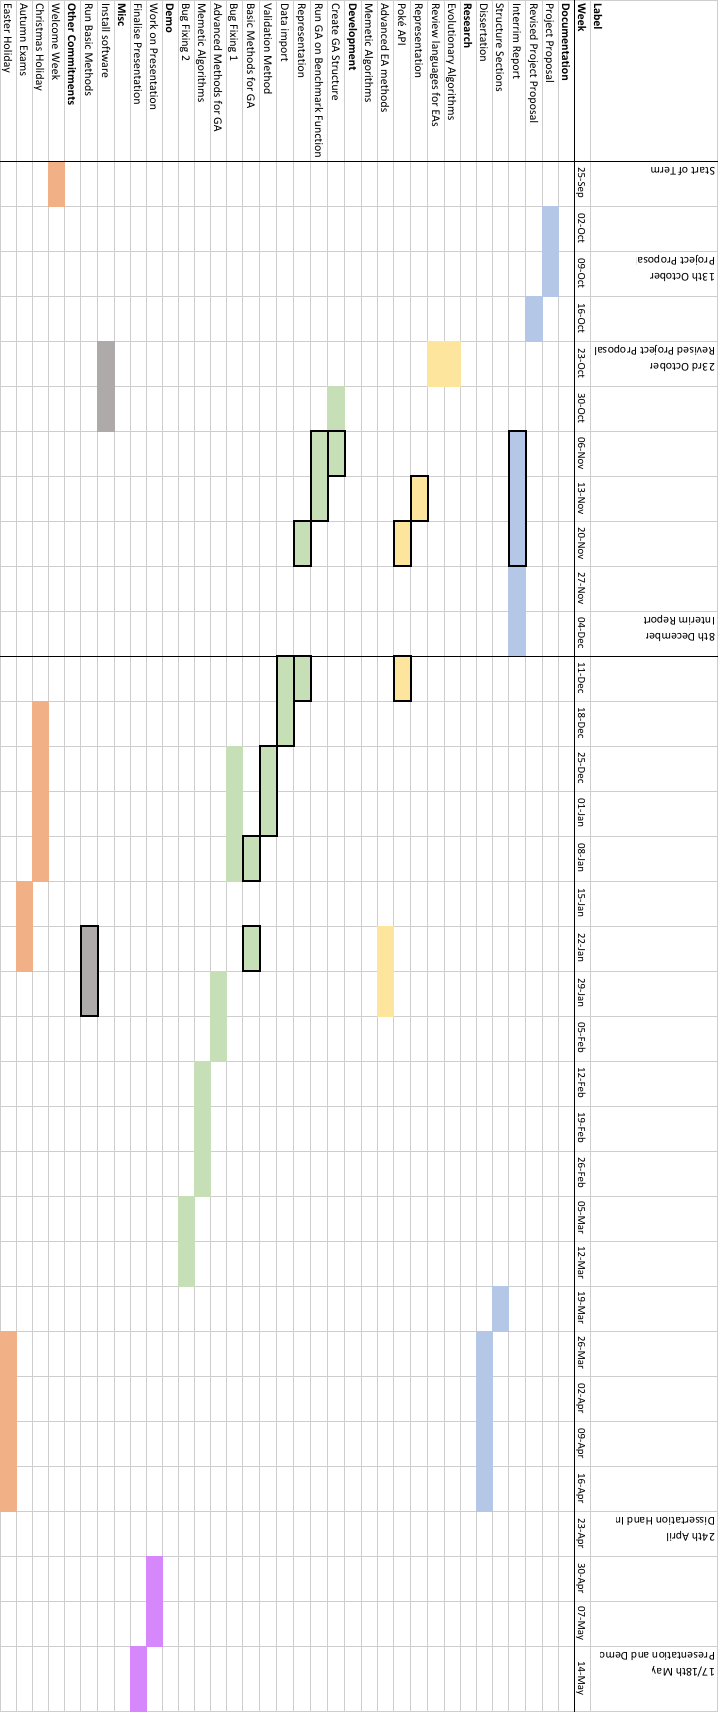
\includegraphics[height=24.8cm]{workPlan.png}
\end{center}


%Bibliography
\subsection{References}
\bibliography{Dissertation}
\bibliographystyle{plain}


\end{document}
